\subsection{The Chessboard Encoding Problem}

This problem is from a collaboration between 3blue1brown and Matt Parker. I attempted this problem years ago, but could not do it, but on a second attempt recently I got it instanteously. I think I spoiled this problem for myself however as I had watched a video recently about a highly relevant problem, and I would never have got it so fast otherwise. I give this problem a difficulty of 5/10, although the ideas behind the solution did lead to someone winning the Turing Prize.

You and a colleague are inprisoned, although the prison warden gives you an opportunity for freedom. There is an $8 \times 8$ chessboard where each square is a hidden compartment, and the warden reveals to one of you, let us call them person A, which square the key to the door is hidden in. A coin is then placed on each square in a configuration decided by the warden that is not known to you or your colleague in advance. Person A has to turn over exactly one coin before leaving the room, at which point person B enters and needs to determine which square has the key. You are allowed to agree a strategy beforehand, although the warden will hear your strategy, and will try and find a configuration of coins to make your strategy not work.

\textbf{Hints:}

\begin{enumerate}
	\item Consider a board with two squares, then four squares.
	\item There exists a reliable strategy if and only if the number of squares is a power of two~\cite{}.
	\item Consider the parity of the number of coins that are heads-up in a region.
\end{enumerate}

\textbf{Solution:}

The solution works by being able to control the parity of the number of heads-up coins in six regions. This produces a six-digit binary number which can be used to encode a square of the chessboard as $8 \times 8 = 64 = 2^6$. The key is to be able to control the parity in each region indepently, and the six regions shown in figure~\ref{fig:TheChessboardEncodingProblem_Grids} allow this.

\begin{figure}[H]
	\begin{center}
		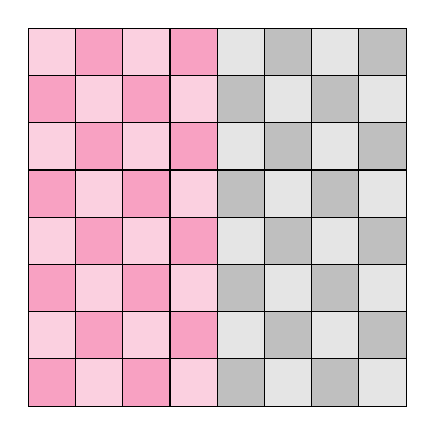
\begin{tikzpicture}[scale=0.6]
			\draw[fill=WildStrawberry, fill opacity=0.4] (0, 0) -- (0, 1) -- (1, 1) -- (1, 0) -- (0, 0);
\draw[fill=WildStrawberry, fill opacity=0.2] (0, 1) -- (0, 2) -- (1, 2) -- (1, 1) -- (0, 1);
\draw[fill=WildStrawberry, fill opacity=0.4] (0, 2) -- (0, 3) -- (1, 3) -- (1, 2) -- (0, 2);
\draw[fill=WildStrawberry, fill opacity=0.2] (0, 3) -- (0, 4) -- (1, 4) -- (1, 3) -- (0, 3);
\draw[fill=WildStrawberry, fill opacity=0.4] (0, 4) -- (0, 5) -- (1, 5) -- (1, 4) -- (0, 4);
\draw[fill=WildStrawberry, fill opacity=0.2] (0, 5) -- (0, 6) -- (1, 6) -- (1, 5) -- (0, 5);
\draw[fill=WildStrawberry, fill opacity=0.4] (0, 6) -- (0, 7) -- (1, 7) -- (1, 6) -- (0, 6);
\draw[fill=WildStrawberry, fill opacity=0.2] (0, 7) -- (0, 8) -- (1, 8) -- (1, 7) -- (0, 7);
\draw[fill=WildStrawberry, fill opacity=0.2] (1, 0) -- (1, 1) -- (2, 1) -- (2, 0) -- (1, 0);
\draw[fill=WildStrawberry, fill opacity=0.4] (1, 1) -- (1, 2) -- (2, 2) -- (2, 1) -- (1, 1);
\draw[fill=WildStrawberry, fill opacity=0.2] (1, 2) -- (1, 3) -- (2, 3) -- (2, 2) -- (1, 2);
\draw[fill=WildStrawberry, fill opacity=0.4] (1, 3) -- (1, 4) -- (2, 4) -- (2, 3) -- (1, 3);
\draw[fill=WildStrawberry, fill opacity=0.2] (1, 4) -- (1, 5) -- (2, 5) -- (2, 4) -- (1, 4);
\draw[fill=WildStrawberry, fill opacity=0.4] (1, 5) -- (1, 6) -- (2, 6) -- (2, 5) -- (1, 5);
\draw[fill=WildStrawberry, fill opacity=0.2] (1, 6) -- (1, 7) -- (2, 7) -- (2, 6) -- (1, 6);
\draw[fill=WildStrawberry, fill opacity=0.4] (1, 7) -- (1, 8) -- (2, 8) -- (2, 7) -- (1, 7);
\draw[fill=WildStrawberry, fill opacity=0.4] (2, 0) -- (2, 1) -- (3, 1) -- (3, 0) -- (2, 0);
\draw[fill=WildStrawberry, fill opacity=0.2] (2, 1) -- (2, 2) -- (3, 2) -- (3, 1) -- (2, 1);
\draw[fill=WildStrawberry, fill opacity=0.4] (2, 2) -- (2, 3) -- (3, 3) -- (3, 2) -- (2, 2);
\draw[fill=WildStrawberry, fill opacity=0.2] (2, 3) -- (2, 4) -- (3, 4) -- (3, 3) -- (2, 3);
\draw[fill=WildStrawberry, fill opacity=0.4] (2, 4) -- (2, 5) -- (3, 5) -- (3, 4) -- (2, 4);
\draw[fill=WildStrawberry, fill opacity=0.2] (2, 5) -- (2, 6) -- (3, 6) -- (3, 5) -- (2, 5);
\draw[fill=WildStrawberry, fill opacity=0.4] (2, 6) -- (2, 7) -- (3, 7) -- (3, 6) -- (2, 6);
\draw[fill=WildStrawberry, fill opacity=0.2] (2, 7) -- (2, 8) -- (3, 8) -- (3, 7) -- (2, 7);
\draw[fill=WildStrawberry, fill opacity=0.2] (3, 0) -- (3, 1) -- (4, 1) -- (4, 0) -- (3, 0);
\draw[fill=WildStrawberry, fill opacity=0.4] (3, 1) -- (3, 2) -- (4, 2) -- (4, 1) -- (3, 1);
\draw[fill=WildStrawberry, fill opacity=0.2] (3, 2) -- (3, 3) -- (4, 3) -- (4, 2) -- (3, 2);
\draw[fill=WildStrawberry, fill opacity=0.4] (3, 3) -- (3, 4) -- (4, 4) -- (4, 3) -- (3, 3);
\draw[fill=WildStrawberry, fill opacity=0.2] (3, 4) -- (3, 5) -- (4, 5) -- (4, 4) -- (3, 4);
\draw[fill=WildStrawberry, fill opacity=0.4] (3, 5) -- (3, 6) -- (4, 6) -- (4, 5) -- (3, 5);
\draw[fill=WildStrawberry, fill opacity=0.2] (3, 6) -- (3, 7) -- (4, 7) -- (4, 6) -- (3, 6);
\draw[fill=WildStrawberry, fill opacity=0.4] (3, 7) -- (3, 8) -- (4, 8) -- (4, 7) -- (3, 7);
\draw[fill=black, fill opacity=0.25] (4, 0) -- (4, 1) -- (5, 1) -- (5, 0) -- (4, 0);
\draw[fill=black, fill opacity=0.1] (4, 1) -- (4, 2) -- (5, 2) -- (5, 1) -- (4, 1);
\draw[fill=black, fill opacity=0.25] (4, 2) -- (4, 3) -- (5, 3) -- (5, 2) -- (4, 2);
\draw[fill=black, fill opacity=0.1] (4, 3) -- (4, 4) -- (5, 4) -- (5, 3) -- (4, 3);
\draw[fill=black, fill opacity=0.25] (4, 4) -- (4, 5) -- (5, 5) -- (5, 4) -- (4, 4);
\draw[fill=black, fill opacity=0.1] (4, 5) -- (4, 6) -- (5, 6) -- (5, 5) -- (4, 5);
\draw[fill=black, fill opacity=0.25] (4, 6) -- (4, 7) -- (5, 7) -- (5, 6) -- (4, 6);
\draw[fill=black, fill opacity=0.1] (4, 7) -- (4, 8) -- (5, 8) -- (5, 7) -- (4, 7);
\draw[fill=black, fill opacity=0.1] (5, 0) -- (5, 1) -- (6, 1) -- (6, 0) -- (5, 0);
\draw[fill=black, fill opacity=0.25] (5, 1) -- (5, 2) -- (6, 2) -- (6, 1) -- (5, 1);
\draw[fill=black, fill opacity=0.1] (5, 2) -- (5, 3) -- (6, 3) -- (6, 2) -- (5, 2);
\draw[fill=black, fill opacity=0.25] (5, 3) -- (5, 4) -- (6, 4) -- (6, 3) -- (5, 3);
\draw[fill=black, fill opacity=0.1] (5, 4) -- (5, 5) -- (6, 5) -- (6, 4) -- (5, 4);
\draw[fill=black, fill opacity=0.25] (5, 5) -- (5, 6) -- (6, 6) -- (6, 5) -- (5, 5);
\draw[fill=black, fill opacity=0.1] (5, 6) -- (5, 7) -- (6, 7) -- (6, 6) -- (5, 6);
\draw[fill=black, fill opacity=0.25] (5, 7) -- (5, 8) -- (6, 8) -- (6, 7) -- (5, 7);
\draw[fill=black, fill opacity=0.25] (6, 0) -- (6, 1) -- (7, 1) -- (7, 0) -- (6, 0);
\draw[fill=black, fill opacity=0.1] (6, 1) -- (6, 2) -- (7, 2) -- (7, 1) -- (6, 1);
\draw[fill=black, fill opacity=0.25] (6, 2) -- (6, 3) -- (7, 3) -- (7, 2) -- (6, 2);
\draw[fill=black, fill opacity=0.1] (6, 3) -- (6, 4) -- (7, 4) -- (7, 3) -- (6, 3);
\draw[fill=black, fill opacity=0.25] (6, 4) -- (6, 5) -- (7, 5) -- (7, 4) -- (6, 4);
\draw[fill=black, fill opacity=0.1] (6, 5) -- (6, 6) -- (7, 6) -- (7, 5) -- (6, 5);
\draw[fill=black, fill opacity=0.25] (6, 6) -- (6, 7) -- (7, 7) -- (7, 6) -- (6, 6);
\draw[fill=black, fill opacity=0.1] (6, 7) -- (6, 8) -- (7, 8) -- (7, 7) -- (6, 7);
\draw[fill=black, fill opacity=0.1] (7, 0) -- (7, 1) -- (8, 1) -- (8, 0) -- (7, 0);
\draw[fill=black, fill opacity=0.25] (7, 1) -- (7, 2) -- (8, 2) -- (8, 1) -- (7, 1);
\draw[fill=black, fill opacity=0.1] (7, 2) -- (7, 3) -- (8, 3) -- (8, 2) -- (7, 2);
\draw[fill=black, fill opacity=0.25] (7, 3) -- (7, 4) -- (8, 4) -- (8, 3) -- (7, 3);
\draw[fill=black, fill opacity=0.1] (7, 4) -- (7, 5) -- (8, 5) -- (8, 4) -- (7, 4);
\draw[fill=black, fill opacity=0.25] (7, 5) -- (7, 6) -- (8, 6) -- (8, 5) -- (7, 5);
\draw[fill=black, fill opacity=0.1] (7, 6) -- (7, 7) -- (8, 7) -- (8, 6) -- (7, 6);
\draw[fill=black, fill opacity=0.25] (7, 7) -- (7, 8) -- (8, 8) -- (8, 7) -- (7, 7);
		\end{tikzpicture}\hspace{5mm}
		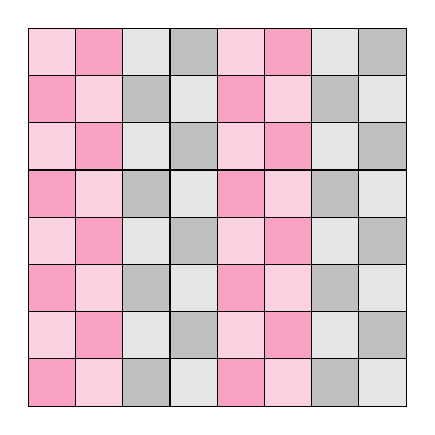
\begin{tikzpicture}[scale=0.6]
			\draw[fill=WildStrawberry, fill opacity=0.4] (0, 0) -- (0, 1) -- (1, 1) -- (1, 0) -- (0, 0);
\draw[fill=WildStrawberry, fill opacity=0.2] (0, 1) -- (0, 2) -- (1, 2) -- (1, 1) -- (0, 1);
\draw[fill=WildStrawberry, fill opacity=0.4] (0, 2) -- (0, 3) -- (1, 3) -- (1, 2) -- (0, 2);
\draw[fill=WildStrawberry, fill opacity=0.2] (0, 3) -- (0, 4) -- (1, 4) -- (1, 3) -- (0, 3);
\draw[fill=WildStrawberry, fill opacity=0.4] (0, 4) -- (0, 5) -- (1, 5) -- (1, 4) -- (0, 4);
\draw[fill=WildStrawberry, fill opacity=0.2] (0, 5) -- (0, 6) -- (1, 6) -- (1, 5) -- (0, 5);
\draw[fill=WildStrawberry, fill opacity=0.4] (0, 6) -- (0, 7) -- (1, 7) -- (1, 6) -- (0, 6);
\draw[fill=WildStrawberry, fill opacity=0.2] (0, 7) -- (0, 8) -- (1, 8) -- (1, 7) -- (0, 7);
\draw[fill=WildStrawberry, fill opacity=0.2] (1, 0) -- (1, 1) -- (2, 1) -- (2, 0) -- (1, 0);
\draw[fill=WildStrawberry, fill opacity=0.4] (1, 1) -- (1, 2) -- (2, 2) -- (2, 1) -- (1, 1);
\draw[fill=WildStrawberry, fill opacity=0.2] (1, 2) -- (1, 3) -- (2, 3) -- (2, 2) -- (1, 2);
\draw[fill=WildStrawberry, fill opacity=0.4] (1, 3) -- (1, 4) -- (2, 4) -- (2, 3) -- (1, 3);
\draw[fill=WildStrawberry, fill opacity=0.2] (1, 4) -- (1, 5) -- (2, 5) -- (2, 4) -- (1, 4);
\draw[fill=WildStrawberry, fill opacity=0.4] (1, 5) -- (1, 6) -- (2, 6) -- (2, 5) -- (1, 5);
\draw[fill=WildStrawberry, fill opacity=0.2] (1, 6) -- (1, 7) -- (2, 7) -- (2, 6) -- (1, 6);
\draw[fill=WildStrawberry, fill opacity=0.4] (1, 7) -- (1, 8) -- (2, 8) -- (2, 7) -- (1, 7);
\draw[fill=black, fill opacity=0.25] (2, 0) -- (2, 1) -- (3, 1) -- (3, 0) -- (2, 0);
\draw[fill=black, fill opacity=0.1] (2, 1) -- (2, 2) -- (3, 2) -- (3, 1) -- (2, 1);
\draw[fill=black, fill opacity=0.25] (2, 2) -- (2, 3) -- (3, 3) -- (3, 2) -- (2, 2);
\draw[fill=black, fill opacity=0.1] (2, 3) -- (2, 4) -- (3, 4) -- (3, 3) -- (2, 3);
\draw[fill=black, fill opacity=0.25] (2, 4) -- (2, 5) -- (3, 5) -- (3, 4) -- (2, 4);
\draw[fill=black, fill opacity=0.1] (2, 5) -- (2, 6) -- (3, 6) -- (3, 5) -- (2, 5);
\draw[fill=black, fill opacity=0.25] (2, 6) -- (2, 7) -- (3, 7) -- (3, 6) -- (2, 6);
\draw[fill=black, fill opacity=0.1] (2, 7) -- (2, 8) -- (3, 8) -- (3, 7) -- (2, 7);
\draw[fill=black, fill opacity=0.1] (3, 0) -- (3, 1) -- (4, 1) -- (4, 0) -- (3, 0);
\draw[fill=black, fill opacity=0.25] (3, 1) -- (3, 2) -- (4, 2) -- (4, 1) -- (3, 1);
\draw[fill=black, fill opacity=0.1] (3, 2) -- (3, 3) -- (4, 3) -- (4, 2) -- (3, 2);
\draw[fill=black, fill opacity=0.25] (3, 3) -- (3, 4) -- (4, 4) -- (4, 3) -- (3, 3);
\draw[fill=black, fill opacity=0.1] (3, 4) -- (3, 5) -- (4, 5) -- (4, 4) -- (3, 4);
\draw[fill=black, fill opacity=0.25] (3, 5) -- (3, 6) -- (4, 6) -- (4, 5) -- (3, 5);
\draw[fill=black, fill opacity=0.1] (3, 6) -- (3, 7) -- (4, 7) -- (4, 6) -- (3, 6);
\draw[fill=black, fill opacity=0.25] (3, 7) -- (3, 8) -- (4, 8) -- (4, 7) -- (3, 7);
\draw[fill=WildStrawberry, fill opacity=0.4] (4, 0) -- (4, 1) -- (5, 1) -- (5, 0) -- (4, 0);
\draw[fill=WildStrawberry, fill opacity=0.2] (4, 1) -- (4, 2) -- (5, 2) -- (5, 1) -- (4, 1);
\draw[fill=WildStrawberry, fill opacity=0.4] (4, 2) -- (4, 3) -- (5, 3) -- (5, 2) -- (4, 2);
\draw[fill=WildStrawberry, fill opacity=0.2] (4, 3) -- (4, 4) -- (5, 4) -- (5, 3) -- (4, 3);
\draw[fill=WildStrawberry, fill opacity=0.4] (4, 4) -- (4, 5) -- (5, 5) -- (5, 4) -- (4, 4);
\draw[fill=WildStrawberry, fill opacity=0.2] (4, 5) -- (4, 6) -- (5, 6) -- (5, 5) -- (4, 5);
\draw[fill=WildStrawberry, fill opacity=0.4] (4, 6) -- (4, 7) -- (5, 7) -- (5, 6) -- (4, 6);
\draw[fill=WildStrawberry, fill opacity=0.2] (4, 7) -- (4, 8) -- (5, 8) -- (5, 7) -- (4, 7);
\draw[fill=WildStrawberry, fill opacity=0.2] (5, 0) -- (5, 1) -- (6, 1) -- (6, 0) -- (5, 0);
\draw[fill=WildStrawberry, fill opacity=0.4] (5, 1) -- (5, 2) -- (6, 2) -- (6, 1) -- (5, 1);
\draw[fill=WildStrawberry, fill opacity=0.2] (5, 2) -- (5, 3) -- (6, 3) -- (6, 2) -- (5, 2);
\draw[fill=WildStrawberry, fill opacity=0.4] (5, 3) -- (5, 4) -- (6, 4) -- (6, 3) -- (5, 3);
\draw[fill=WildStrawberry, fill opacity=0.2] (5, 4) -- (5, 5) -- (6, 5) -- (6, 4) -- (5, 4);
\draw[fill=WildStrawberry, fill opacity=0.4] (5, 5) -- (5, 6) -- (6, 6) -- (6, 5) -- (5, 5);
\draw[fill=WildStrawberry, fill opacity=0.2] (5, 6) -- (5, 7) -- (6, 7) -- (6, 6) -- (5, 6);
\draw[fill=WildStrawberry, fill opacity=0.4] (5, 7) -- (5, 8) -- (6, 8) -- (6, 7) -- (5, 7);
\draw[fill=black, fill opacity=0.25] (6, 0) -- (6, 1) -- (7, 1) -- (7, 0) -- (6, 0);
\draw[fill=black, fill opacity=0.1] (6, 1) -- (6, 2) -- (7, 2) -- (7, 1) -- (6, 1);
\draw[fill=black, fill opacity=0.25] (6, 2) -- (6, 3) -- (7, 3) -- (7, 2) -- (6, 2);
\draw[fill=black, fill opacity=0.1] (6, 3) -- (6, 4) -- (7, 4) -- (7, 3) -- (6, 3);
\draw[fill=black, fill opacity=0.25] (6, 4) -- (6, 5) -- (7, 5) -- (7, 4) -- (6, 4);
\draw[fill=black, fill opacity=0.1] (6, 5) -- (6, 6) -- (7, 6) -- (7, 5) -- (6, 5);
\draw[fill=black, fill opacity=0.25] (6, 6) -- (6, 7) -- (7, 7) -- (7, 6) -- (6, 6);
\draw[fill=black, fill opacity=0.1] (6, 7) -- (6, 8) -- (7, 8) -- (7, 7) -- (6, 7);
\draw[fill=black, fill opacity=0.1] (7, 0) -- (7, 1) -- (8, 1) -- (8, 0) -- (7, 0);
\draw[fill=black, fill opacity=0.25] (7, 1) -- (7, 2) -- (8, 2) -- (8, 1) -- (7, 1);
\draw[fill=black, fill opacity=0.1] (7, 2) -- (7, 3) -- (8, 3) -- (8, 2) -- (7, 2);
\draw[fill=black, fill opacity=0.25] (7, 3) -- (7, 4) -- (8, 4) -- (8, 3) -- (7, 3);
\draw[fill=black, fill opacity=0.1] (7, 4) -- (7, 5) -- (8, 5) -- (8, 4) -- (7, 4);
\draw[fill=black, fill opacity=0.25] (7, 5) -- (7, 6) -- (8, 6) -- (8, 5) -- (7, 5);
\draw[fill=black, fill opacity=0.1] (7, 6) -- (7, 7) -- (8, 7) -- (8, 6) -- (7, 6);
\draw[fill=black, fill opacity=0.25] (7, 7) -- (7, 8) -- (8, 8) -- (8, 7) -- (7, 7);
		\end{tikzpicture}\hspace{5mm}
		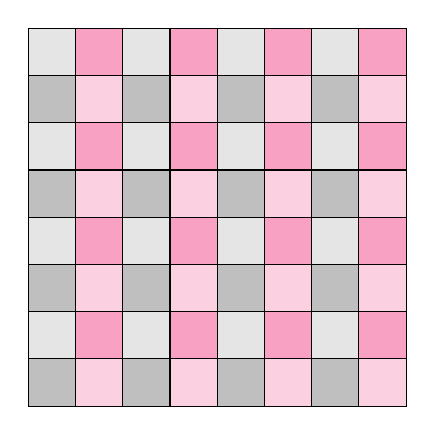
\begin{tikzpicture}[scale=0.6]
			\draw[fill=black, fill opacity=0.25] (0, 0) -- (0, 1) -- (1, 1) -- (1, 0) -- (0, 0);
\draw[fill=WildStrawberry, fill opacity=0.2] (1, 0) -- (1, 1) -- (2, 1) -- (2, 0) -- (1, 0);
\draw[fill=black, fill opacity=0.25] (2, 0) -- (2, 1) -- (3, 1) -- (3, 0) -- (2, 0);
\draw[fill=WildStrawberry, fill opacity=0.2] (3, 0) -- (3, 1) -- (4, 1) -- (4, 0) -- (3, 0);
\draw[fill=black, fill opacity=0.25] (4, 0) -- (4, 1) -- (5, 1) -- (5, 0) -- (4, 0);
\draw[fill=WildStrawberry, fill opacity=0.2] (5, 0) -- (5, 1) -- (6, 1) -- (6, 0) -- (5, 0);
\draw[fill=black, fill opacity=0.25] (6, 0) -- (6, 1) -- (7, 1) -- (7, 0) -- (6, 0);
\draw[fill=WildStrawberry, fill opacity=0.2] (7, 0) -- (7, 1) -- (8, 1) -- (8, 0) -- (7, 0);
\draw[fill=black, fill opacity=0.1] (0, 1) -- (0, 2) -- (1, 2) -- (1, 1) -- (0, 1);
\draw[fill=WildStrawberry, fill opacity=0.4] (1, 1) -- (1, 2) -- (2, 2) -- (2, 1) -- (1, 1);
\draw[fill=black, fill opacity=0.1] (2, 1) -- (2, 2) -- (3, 2) -- (3, 1) -- (2, 1);
\draw[fill=WildStrawberry, fill opacity=0.4] (3, 1) -- (3, 2) -- (4, 2) -- (4, 1) -- (3, 1);
\draw[fill=black, fill opacity=0.1] (4, 1) -- (4, 2) -- (5, 2) -- (5, 1) -- (4, 1);
\draw[fill=WildStrawberry, fill opacity=0.4] (5, 1) -- (5, 2) -- (6, 2) -- (6, 1) -- (5, 1);
\draw[fill=black, fill opacity=0.1] (6, 1) -- (6, 2) -- (7, 2) -- (7, 1) -- (6, 1);
\draw[fill=WildStrawberry, fill opacity=0.4] (7, 1) -- (7, 2) -- (8, 2) -- (8, 1) -- (7, 1);
\draw[fill=black, fill opacity=0.25] (0, 2) -- (0, 3) -- (1, 3) -- (1, 2) -- (0, 2);
\draw[fill=WildStrawberry, fill opacity=0.2] (1, 2) -- (1, 3) -- (2, 3) -- (2, 2) -- (1, 2);
\draw[fill=black, fill opacity=0.25] (2, 2) -- (2, 3) -- (3, 3) -- (3, 2) -- (2, 2);
\draw[fill=WildStrawberry, fill opacity=0.2] (3, 2) -- (3, 3) -- (4, 3) -- (4, 2) -- (3, 2);
\draw[fill=black, fill opacity=0.25] (4, 2) -- (4, 3) -- (5, 3) -- (5, 2) -- (4, 2);
\draw[fill=WildStrawberry, fill opacity=0.2] (5, 2) -- (5, 3) -- (6, 3) -- (6, 2) -- (5, 2);
\draw[fill=black, fill opacity=0.25] (6, 2) -- (6, 3) -- (7, 3) -- (7, 2) -- (6, 2);
\draw[fill=WildStrawberry, fill opacity=0.2] (7, 2) -- (7, 3) -- (8, 3) -- (8, 2) -- (7, 2);
\draw[fill=black, fill opacity=0.1] (0, 3) -- (0, 4) -- (1, 4) -- (1, 3) -- (0, 3);
\draw[fill=WildStrawberry, fill opacity=0.4] (1, 3) -- (1, 4) -- (2, 4) -- (2, 3) -- (1, 3);
\draw[fill=black, fill opacity=0.1] (2, 3) -- (2, 4) -- (3, 4) -- (3, 3) -- (2, 3);
\draw[fill=WildStrawberry, fill opacity=0.4] (3, 3) -- (3, 4) -- (4, 4) -- (4, 3) -- (3, 3);
\draw[fill=black, fill opacity=0.1] (4, 3) -- (4, 4) -- (5, 4) -- (5, 3) -- (4, 3);
\draw[fill=WildStrawberry, fill opacity=0.4] (5, 3) -- (5, 4) -- (6, 4) -- (6, 3) -- (5, 3);
\draw[fill=black, fill opacity=0.1] (6, 3) -- (6, 4) -- (7, 4) -- (7, 3) -- (6, 3);
\draw[fill=WildStrawberry, fill opacity=0.4] (7, 3) -- (7, 4) -- (8, 4) -- (8, 3) -- (7, 3);
\draw[fill=black, fill opacity=0.25] (0, 4) -- (0, 5) -- (1, 5) -- (1, 4) -- (0, 4);
\draw[fill=WildStrawberry, fill opacity=0.2] (1, 4) -- (1, 5) -- (2, 5) -- (2, 4) -- (1, 4);
\draw[fill=black, fill opacity=0.25] (2, 4) -- (2, 5) -- (3, 5) -- (3, 4) -- (2, 4);
\draw[fill=WildStrawberry, fill opacity=0.2] (3, 4) -- (3, 5) -- (4, 5) -- (4, 4) -- (3, 4);
\draw[fill=black, fill opacity=0.25] (4, 4) -- (4, 5) -- (5, 5) -- (5, 4) -- (4, 4);
\draw[fill=WildStrawberry, fill opacity=0.2] (5, 4) -- (5, 5) -- (6, 5) -- (6, 4) -- (5, 4);
\draw[fill=black, fill opacity=0.25] (6, 4) -- (6, 5) -- (7, 5) -- (7, 4) -- (6, 4);
\draw[fill=WildStrawberry, fill opacity=0.2] (7, 4) -- (7, 5) -- (8, 5) -- (8, 4) -- (7, 4);
\draw[fill=black, fill opacity=0.1] (0, 5) -- (0, 6) -- (1, 6) -- (1, 5) -- (0, 5);
\draw[fill=WildStrawberry, fill opacity=0.4] (1, 5) -- (1, 6) -- (2, 6) -- (2, 5) -- (1, 5);
\draw[fill=black, fill opacity=0.1] (2, 5) -- (2, 6) -- (3, 6) -- (3, 5) -- (2, 5);
\draw[fill=WildStrawberry, fill opacity=0.4] (3, 5) -- (3, 6) -- (4, 6) -- (4, 5) -- (3, 5);
\draw[fill=black, fill opacity=0.1] (4, 5) -- (4, 6) -- (5, 6) -- (5, 5) -- (4, 5);
\draw[fill=WildStrawberry, fill opacity=0.4] (5, 5) -- (5, 6) -- (6, 6) -- (6, 5) -- (5, 5);
\draw[fill=black, fill opacity=0.1] (6, 5) -- (6, 6) -- (7, 6) -- (7, 5) -- (6, 5);
\draw[fill=WildStrawberry, fill opacity=0.4] (7, 5) -- (7, 6) -- (8, 6) -- (8, 5) -- (7, 5);
\draw[fill=black, fill opacity=0.25] (0, 6) -- (0, 7) -- (1, 7) -- (1, 6) -- (0, 6);
\draw[fill=WildStrawberry, fill opacity=0.2] (1, 6) -- (1, 7) -- (2, 7) -- (2, 6) -- (1, 6);
\draw[fill=black, fill opacity=0.25] (2, 6) -- (2, 7) -- (3, 7) -- (3, 6) -- (2, 6);
\draw[fill=WildStrawberry, fill opacity=0.2] (3, 6) -- (3, 7) -- (4, 7) -- (4, 6) -- (3, 6);
\draw[fill=black, fill opacity=0.25] (4, 6) -- (4, 7) -- (5, 7) -- (5, 6) -- (4, 6);
\draw[fill=WildStrawberry, fill opacity=0.2] (5, 6) -- (5, 7) -- (6, 7) -- (6, 6) -- (5, 6);
\draw[fill=black, fill opacity=0.25] (6, 6) -- (6, 7) -- (7, 7) -- (7, 6) -- (6, 6);
\draw[fill=WildStrawberry, fill opacity=0.2] (7, 6) -- (7, 7) -- (8, 7) -- (8, 6) -- (7, 6);
\draw[fill=black, fill opacity=0.1] (0, 7) -- (0, 8) -- (1, 8) -- (1, 7) -- (0, 7);
\draw[fill=WildStrawberry, fill opacity=0.4] (1, 7) -- (1, 8) -- (2, 8) -- (2, 7) -- (1, 7);
\draw[fill=black, fill opacity=0.1] (2, 7) -- (2, 8) -- (3, 8) -- (3, 7) -- (2, 7);
\draw[fill=WildStrawberry, fill opacity=0.4] (3, 7) -- (3, 8) -- (4, 8) -- (4, 7) -- (3, 7);
\draw[fill=black, fill opacity=0.1] (4, 7) -- (4, 8) -- (5, 8) -- (5, 7) -- (4, 7);
\draw[fill=WildStrawberry, fill opacity=0.4] (5, 7) -- (5, 8) -- (6, 8) -- (6, 7) -- (5, 7);
\draw[fill=black, fill opacity=0.1] (6, 7) -- (6, 8) -- (7, 8) -- (7, 7) -- (6, 7);
\draw[fill=WildStrawberry, fill opacity=0.4] (7, 7) -- (7, 8) -- (8, 8) -- (8, 7) -- (7, 7);
		\end{tikzpicture}\vspace{6mm}
		\\
		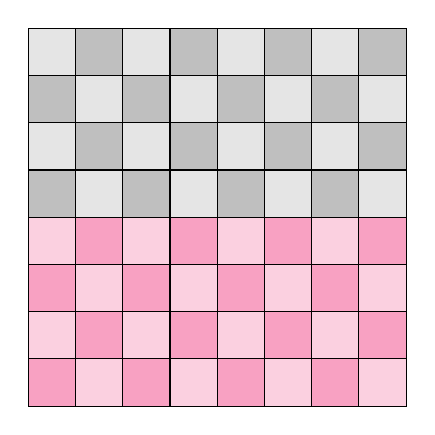
\begin{tikzpicture}[scale=0.6]
			\draw[fill=WildStrawberry, fill opacity=0.4] (0, 0) -- (0, 1) -- (1, 1) -- (1, 0) -- (0, 0);
\draw[fill=WildStrawberry, fill opacity=0.2] (1, 0) -- (1, 1) -- (2, 1) -- (2, 0) -- (1, 0);
\draw[fill=WildStrawberry, fill opacity=0.4] (2, 0) -- (2, 1) -- (3, 1) -- (3, 0) -- (2, 0);
\draw[fill=WildStrawberry, fill opacity=0.2] (3, 0) -- (3, 1) -- (4, 1) -- (4, 0) -- (3, 0);
\draw[fill=WildStrawberry, fill opacity=0.4] (4, 0) -- (4, 1) -- (5, 1) -- (5, 0) -- (4, 0);
\draw[fill=WildStrawberry, fill opacity=0.2] (5, 0) -- (5, 1) -- (6, 1) -- (6, 0) -- (5, 0);
\draw[fill=WildStrawberry, fill opacity=0.4] (6, 0) -- (6, 1) -- (7, 1) -- (7, 0) -- (6, 0);
\draw[fill=WildStrawberry, fill opacity=0.2] (7, 0) -- (7, 1) -- (8, 1) -- (8, 0) -- (7, 0);
\draw[fill=WildStrawberry, fill opacity=0.2] (0, 1) -- (0, 2) -- (1, 2) -- (1, 1) -- (0, 1);
\draw[fill=WildStrawberry, fill opacity=0.4] (1, 1) -- (1, 2) -- (2, 2) -- (2, 1) -- (1, 1);
\draw[fill=WildStrawberry, fill opacity=0.2] (2, 1) -- (2, 2) -- (3, 2) -- (3, 1) -- (2, 1);
\draw[fill=WildStrawberry, fill opacity=0.4] (3, 1) -- (3, 2) -- (4, 2) -- (4, 1) -- (3, 1);
\draw[fill=WildStrawberry, fill opacity=0.2] (4, 1) -- (4, 2) -- (5, 2) -- (5, 1) -- (4, 1);
\draw[fill=WildStrawberry, fill opacity=0.4] (5, 1) -- (5, 2) -- (6, 2) -- (6, 1) -- (5, 1);
\draw[fill=WildStrawberry, fill opacity=0.2] (6, 1) -- (6, 2) -- (7, 2) -- (7, 1) -- (6, 1);
\draw[fill=WildStrawberry, fill opacity=0.4] (7, 1) -- (7, 2) -- (8, 2) -- (8, 1) -- (7, 1);
\draw[fill=WildStrawberry, fill opacity=0.4] (0, 2) -- (0, 3) -- (1, 3) -- (1, 2) -- (0, 2);
\draw[fill=WildStrawberry, fill opacity=0.2] (1, 2) -- (1, 3) -- (2, 3) -- (2, 2) -- (1, 2);
\draw[fill=WildStrawberry, fill opacity=0.4] (2, 2) -- (2, 3) -- (3, 3) -- (3, 2) -- (2, 2);
\draw[fill=WildStrawberry, fill opacity=0.2] (3, 2) -- (3, 3) -- (4, 3) -- (4, 2) -- (3, 2);
\draw[fill=WildStrawberry, fill opacity=0.4] (4, 2) -- (4, 3) -- (5, 3) -- (5, 2) -- (4, 2);
\draw[fill=WildStrawberry, fill opacity=0.2] (5, 2) -- (5, 3) -- (6, 3) -- (6, 2) -- (5, 2);
\draw[fill=WildStrawberry, fill opacity=0.4] (6, 2) -- (6, 3) -- (7, 3) -- (7, 2) -- (6, 2);
\draw[fill=WildStrawberry, fill opacity=0.2] (7, 2) -- (7, 3) -- (8, 3) -- (8, 2) -- (7, 2);
\draw[fill=WildStrawberry, fill opacity=0.2] (0, 3) -- (0, 4) -- (1, 4) -- (1, 3) -- (0, 3);
\draw[fill=WildStrawberry, fill opacity=0.4] (1, 3) -- (1, 4) -- (2, 4) -- (2, 3) -- (1, 3);
\draw[fill=WildStrawberry, fill opacity=0.2] (2, 3) -- (2, 4) -- (3, 4) -- (3, 3) -- (2, 3);
\draw[fill=WildStrawberry, fill opacity=0.4] (3, 3) -- (3, 4) -- (4, 4) -- (4, 3) -- (3, 3);
\draw[fill=WildStrawberry, fill opacity=0.2] (4, 3) -- (4, 4) -- (5, 4) -- (5, 3) -- (4, 3);
\draw[fill=WildStrawberry, fill opacity=0.4] (5, 3) -- (5, 4) -- (6, 4) -- (6, 3) -- (5, 3);
\draw[fill=WildStrawberry, fill opacity=0.2] (6, 3) -- (6, 4) -- (7, 4) -- (7, 3) -- (6, 3);
\draw[fill=WildStrawberry, fill opacity=0.4] (7, 3) -- (7, 4) -- (8, 4) -- (8, 3) -- (7, 3);
\draw[fill=black, fill opacity=0.25] (0, 4) -- (0, 5) -- (1, 5) -- (1, 4) -- (0, 4);
\draw[fill=black, fill opacity=0.1] (1, 4) -- (1, 5) -- (2, 5) -- (2, 4) -- (1, 4);
\draw[fill=black, fill opacity=0.25] (2, 4) -- (2, 5) -- (3, 5) -- (3, 4) -- (2, 4);
\draw[fill=black, fill opacity=0.1] (3, 4) -- (3, 5) -- (4, 5) -- (4, 4) -- (3, 4);
\draw[fill=black, fill opacity=0.25] (4, 4) -- (4, 5) -- (5, 5) -- (5, 4) -- (4, 4);
\draw[fill=black, fill opacity=0.1] (5, 4) -- (5, 5) -- (6, 5) -- (6, 4) -- (5, 4);
\draw[fill=black, fill opacity=0.25] (6, 4) -- (6, 5) -- (7, 5) -- (7, 4) -- (6, 4);
\draw[fill=black, fill opacity=0.1] (7, 4) -- (7, 5) -- (8, 5) -- (8, 4) -- (7, 4);
\draw[fill=black, fill opacity=0.1] (0, 5) -- (0, 6) -- (1, 6) -- (1, 5) -- (0, 5);
\draw[fill=black, fill opacity=0.25] (1, 5) -- (1, 6) -- (2, 6) -- (2, 5) -- (1, 5);
\draw[fill=black, fill opacity=0.1] (2, 5) -- (2, 6) -- (3, 6) -- (3, 5) -- (2, 5);
\draw[fill=black, fill opacity=0.25] (3, 5) -- (3, 6) -- (4, 6) -- (4, 5) -- (3, 5);
\draw[fill=black, fill opacity=0.1] (4, 5) -- (4, 6) -- (5, 6) -- (5, 5) -- (4, 5);
\draw[fill=black, fill opacity=0.25] (5, 5) -- (5, 6) -- (6, 6) -- (6, 5) -- (5, 5);
\draw[fill=black, fill opacity=0.1] (6, 5) -- (6, 6) -- (7, 6) -- (7, 5) -- (6, 5);
\draw[fill=black, fill opacity=0.25] (7, 5) -- (7, 6) -- (8, 6) -- (8, 5) -- (7, 5);
\draw[fill=black, fill opacity=0.25] (0, 6) -- (0, 7) -- (1, 7) -- (1, 6) -- (0, 6);
\draw[fill=black, fill opacity=0.1] (1, 6) -- (1, 7) -- (2, 7) -- (2, 6) -- (1, 6);
\draw[fill=black, fill opacity=0.25] (2, 6) -- (2, 7) -- (3, 7) -- (3, 6) -- (2, 6);
\draw[fill=black, fill opacity=0.1] (3, 6) -- (3, 7) -- (4, 7) -- (4, 6) -- (3, 6);
\draw[fill=black, fill opacity=0.25] (4, 6) -- (4, 7) -- (5, 7) -- (5, 6) -- (4, 6);
\draw[fill=black, fill opacity=0.1] (5, 6) -- (5, 7) -- (6, 7) -- (6, 6) -- (5, 6);
\draw[fill=black, fill opacity=0.25] (6, 6) -- (6, 7) -- (7, 7) -- (7, 6) -- (6, 6);
\draw[fill=black, fill opacity=0.1] (7, 6) -- (7, 7) -- (8, 7) -- (8, 6) -- (7, 6);
\draw[fill=black, fill opacity=0.1] (0, 7) -- (0, 8) -- (1, 8) -- (1, 7) -- (0, 7);
\draw[fill=black, fill opacity=0.25] (1, 7) -- (1, 8) -- (2, 8) -- (2, 7) -- (1, 7);
\draw[fill=black, fill opacity=0.1] (2, 7) -- (2, 8) -- (3, 8) -- (3, 7) -- (2, 7);
\draw[fill=black, fill opacity=0.25] (3, 7) -- (3, 8) -- (4, 8) -- (4, 7) -- (3, 7);
\draw[fill=black, fill opacity=0.1] (4, 7) -- (4, 8) -- (5, 8) -- (5, 7) -- (4, 7);
\draw[fill=black, fill opacity=0.25] (5, 7) -- (5, 8) -- (6, 8) -- (6, 7) -- (5, 7);
\draw[fill=black, fill opacity=0.1] (6, 7) -- (6, 8) -- (7, 8) -- (7, 7) -- (6, 7);
\draw[fill=black, fill opacity=0.25] (7, 7) -- (7, 8) -- (8, 8) -- (8, 7) -- (7, 7);
		\end{tikzpicture}\hspace{5mm}
		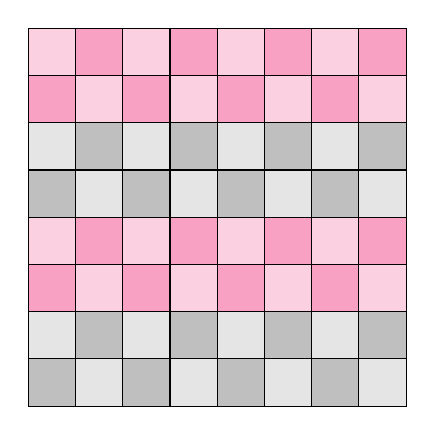
\begin{tikzpicture}[scale=0.6]
			\draw[fill=black, fill opacity=0.25] (0, 0) -- (0, 1) -- (1, 1) -- (1, 0) -- (0, 0);
\draw[fill=black, fill opacity=0.1] (0, 1) -- (0, 2) -- (1, 2) -- (1, 1) -- (0, 1);
\draw[fill=WildStrawberry, fill opacity=0.4] (0, 2) -- (0, 3) -- (1, 3) -- (1, 2) -- (0, 2);
\draw[fill=WildStrawberry, fill opacity=0.2] (0, 3) -- (0, 4) -- (1, 4) -- (1, 3) -- (0, 3);
\draw[fill=black, fill opacity=0.25] (0, 4) -- (0, 5) -- (1, 5) -- (1, 4) -- (0, 4);
\draw[fill=black, fill opacity=0.1] (0, 5) -- (0, 6) -- (1, 6) -- (1, 5) -- (0, 5);
\draw[fill=WildStrawberry, fill opacity=0.4] (0, 6) -- (0, 7) -- (1, 7) -- (1, 6) -- (0, 6);
\draw[fill=WildStrawberry, fill opacity=0.2] (0, 7) -- (0, 8) -- (1, 8) -- (1, 7) -- (0, 7);
\draw[fill=black, fill opacity=0.1] (1, 0) -- (1, 1) -- (2, 1) -- (2, 0) -- (1, 0);
\draw[fill=black, fill opacity=0.25] (1, 1) -- (1, 2) -- (2, 2) -- (2, 1) -- (1, 1);
\draw[fill=WildStrawberry, fill opacity=0.2] (1, 2) -- (1, 3) -- (2, 3) -- (2, 2) -- (1, 2);
\draw[fill=WildStrawberry, fill opacity=0.4] (1, 3) -- (1, 4) -- (2, 4) -- (2, 3) -- (1, 3);
\draw[fill=black, fill opacity=0.1] (1, 4) -- (1, 5) -- (2, 5) -- (2, 4) -- (1, 4);
\draw[fill=black, fill opacity=0.25] (1, 5) -- (1, 6) -- (2, 6) -- (2, 5) -- (1, 5);
\draw[fill=WildStrawberry, fill opacity=0.2] (1, 6) -- (1, 7) -- (2, 7) -- (2, 6) -- (1, 6);
\draw[fill=WildStrawberry, fill opacity=0.4] (1, 7) -- (1, 8) -- (2, 8) -- (2, 7) -- (1, 7);
\draw[fill=black, fill opacity=0.25] (2, 0) -- (2, 1) -- (3, 1) -- (3, 0) -- (2, 0);
\draw[fill=black, fill opacity=0.1] (2, 1) -- (2, 2) -- (3, 2) -- (3, 1) -- (2, 1);
\draw[fill=WildStrawberry, fill opacity=0.4] (2, 2) -- (2, 3) -- (3, 3) -- (3, 2) -- (2, 2);
\draw[fill=WildStrawberry, fill opacity=0.2] (2, 3) -- (2, 4) -- (3, 4) -- (3, 3) -- (2, 3);
\draw[fill=black, fill opacity=0.25] (2, 4) -- (2, 5) -- (3, 5) -- (3, 4) -- (2, 4);
\draw[fill=black, fill opacity=0.1] (2, 5) -- (2, 6) -- (3, 6) -- (3, 5) -- (2, 5);
\draw[fill=WildStrawberry, fill opacity=0.4] (2, 6) -- (2, 7) -- (3, 7) -- (3, 6) -- (2, 6);
\draw[fill=WildStrawberry, fill opacity=0.2] (2, 7) -- (2, 8) -- (3, 8) -- (3, 7) -- (2, 7);
\draw[fill=black, fill opacity=0.1] (3, 0) -- (3, 1) -- (4, 1) -- (4, 0) -- (3, 0);
\draw[fill=black, fill opacity=0.25] (3, 1) -- (3, 2) -- (4, 2) -- (4, 1) -- (3, 1);
\draw[fill=WildStrawberry, fill opacity=0.2] (3, 2) -- (3, 3) -- (4, 3) -- (4, 2) -- (3, 2);
\draw[fill=WildStrawberry, fill opacity=0.4] (3, 3) -- (3, 4) -- (4, 4) -- (4, 3) -- (3, 3);
\draw[fill=black, fill opacity=0.1] (3, 4) -- (3, 5) -- (4, 5) -- (4, 4) -- (3, 4);
\draw[fill=black, fill opacity=0.25] (3, 5) -- (3, 6) -- (4, 6) -- (4, 5) -- (3, 5);
\draw[fill=WildStrawberry, fill opacity=0.2] (3, 6) -- (3, 7) -- (4, 7) -- (4, 6) -- (3, 6);
\draw[fill=WildStrawberry, fill opacity=0.4] (3, 7) -- (3, 8) -- (4, 8) -- (4, 7) -- (3, 7);
\draw[fill=black, fill opacity=0.25] (4, 0) -- (4, 1) -- (5, 1) -- (5, 0) -- (4, 0);
\draw[fill=black, fill opacity=0.1] (4, 1) -- (4, 2) -- (5, 2) -- (5, 1) -- (4, 1);
\draw[fill=WildStrawberry, fill opacity=0.4] (4, 2) -- (4, 3) -- (5, 3) -- (5, 2) -- (4, 2);
\draw[fill=WildStrawberry, fill opacity=0.2] (4, 3) -- (4, 4) -- (5, 4) -- (5, 3) -- (4, 3);
\draw[fill=black, fill opacity=0.25] (4, 4) -- (4, 5) -- (5, 5) -- (5, 4) -- (4, 4);
\draw[fill=black, fill opacity=0.1] (4, 5) -- (4, 6) -- (5, 6) -- (5, 5) -- (4, 5);
\draw[fill=WildStrawberry, fill opacity=0.4] (4, 6) -- (4, 7) -- (5, 7) -- (5, 6) -- (4, 6);
\draw[fill=WildStrawberry, fill opacity=0.2] (4, 7) -- (4, 8) -- (5, 8) -- (5, 7) -- (4, 7);
\draw[fill=black, fill opacity=0.1] (5, 0) -- (5, 1) -- (6, 1) -- (6, 0) -- (5, 0);
\draw[fill=black, fill opacity=0.25] (5, 1) -- (5, 2) -- (6, 2) -- (6, 1) -- (5, 1);
\draw[fill=WildStrawberry, fill opacity=0.2] (5, 2) -- (5, 3) -- (6, 3) -- (6, 2) -- (5, 2);
\draw[fill=WildStrawberry, fill opacity=0.4] (5, 3) -- (5, 4) -- (6, 4) -- (6, 3) -- (5, 3);
\draw[fill=black, fill opacity=0.1] (5, 4) -- (5, 5) -- (6, 5) -- (6, 4) -- (5, 4);
\draw[fill=black, fill opacity=0.25] (5, 5) -- (5, 6) -- (6, 6) -- (6, 5) -- (5, 5);
\draw[fill=WildStrawberry, fill opacity=0.2] (5, 6) -- (5, 7) -- (6, 7) -- (6, 6) -- (5, 6);
\draw[fill=WildStrawberry, fill opacity=0.4] (5, 7) -- (5, 8) -- (6, 8) -- (6, 7) -- (5, 7);
\draw[fill=black, fill opacity=0.25] (6, 0) -- (6, 1) -- (7, 1) -- (7, 0) -- (6, 0);
\draw[fill=black, fill opacity=0.1] (6, 1) -- (6, 2) -- (7, 2) -- (7, 1) -- (6, 1);
\draw[fill=WildStrawberry, fill opacity=0.4] (6, 2) -- (6, 3) -- (7, 3) -- (7, 2) -- (6, 2);
\draw[fill=WildStrawberry, fill opacity=0.2] (6, 3) -- (6, 4) -- (7, 4) -- (7, 3) -- (6, 3);
\draw[fill=black, fill opacity=0.25] (6, 4) -- (6, 5) -- (7, 5) -- (7, 4) -- (6, 4);
\draw[fill=black, fill opacity=0.1] (6, 5) -- (6, 6) -- (7, 6) -- (7, 5) -- (6, 5);
\draw[fill=WildStrawberry, fill opacity=0.4] (6, 6) -- (6, 7) -- (7, 7) -- (7, 6) -- (6, 6);
\draw[fill=WildStrawberry, fill opacity=0.2] (6, 7) -- (6, 8) -- (7, 8) -- (7, 7) -- (6, 7);
\draw[fill=black, fill opacity=0.1] (7, 0) -- (7, 1) -- (8, 1) -- (8, 0) -- (7, 0);
\draw[fill=black, fill opacity=0.25] (7, 1) -- (7, 2) -- (8, 2) -- (8, 1) -- (7, 1);
\draw[fill=WildStrawberry, fill opacity=0.2] (7, 2) -- (7, 3) -- (8, 3) -- (8, 2) -- (7, 2);
\draw[fill=WildStrawberry, fill opacity=0.4] (7, 3) -- (7, 4) -- (8, 4) -- (8, 3) -- (7, 3);
\draw[fill=black, fill opacity=0.1] (7, 4) -- (7, 5) -- (8, 5) -- (8, 4) -- (7, 4);
\draw[fill=black, fill opacity=0.25] (7, 5) -- (7, 6) -- (8, 6) -- (8, 5) -- (7, 5);
\draw[fill=WildStrawberry, fill opacity=0.2] (7, 6) -- (7, 7) -- (8, 7) -- (8, 6) -- (7, 6);
\draw[fill=WildStrawberry, fill opacity=0.4] (7, 7) -- (7, 8) -- (8, 8) -- (8, 7) -- (7, 7);
		\end{tikzpicture}\hspace{5mm}
		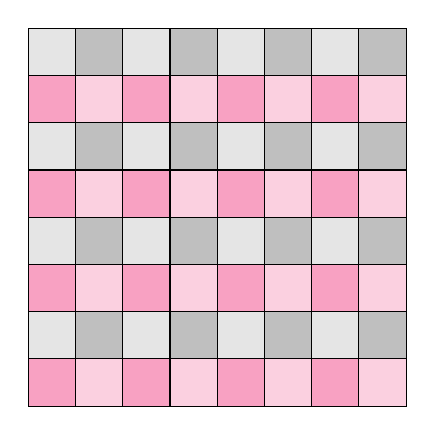
\begin{tikzpicture}[scale=0.6]
			\draw[fill=WildStrawberry, fill opacity=0.4] (0, 0) -- (0, 1) -- (1, 1) -- (1, 0) -- (0, 0);
\draw[fill=WildStrawberry, fill opacity=0.2] (1, 0) -- (1, 1) -- (2, 1) -- (2, 0) -- (1, 0);
\draw[fill=WildStrawberry, fill opacity=0.4] (2, 0) -- (2, 1) -- (3, 1) -- (3, 0) -- (2, 0);
\draw[fill=WildStrawberry, fill opacity=0.2] (3, 0) -- (3, 1) -- (4, 1) -- (4, 0) -- (3, 0);
\draw[fill=WildStrawberry, fill opacity=0.4] (4, 0) -- (4, 1) -- (5, 1) -- (5, 0) -- (4, 0);
\draw[fill=WildStrawberry, fill opacity=0.2] (5, 0) -- (5, 1) -- (6, 1) -- (6, 0) -- (5, 0);
\draw[fill=WildStrawberry, fill opacity=0.4] (6, 0) -- (6, 1) -- (7, 1) -- (7, 0) -- (6, 0);
\draw[fill=WildStrawberry, fill opacity=0.2] (7, 0) -- (7, 1) -- (8, 1) -- (8, 0) -- (7, 0);
\draw[fill=black, fill opacity=0.1] (0, 1) -- (0, 2) -- (1, 2) -- (1, 1) -- (0, 1);
\draw[fill=black, fill opacity=0.25] (1, 1) -- (1, 2) -- (2, 2) -- (2, 1) -- (1, 1);
\draw[fill=black, fill opacity=0.1] (2, 1) -- (2, 2) -- (3, 2) -- (3, 1) -- (2, 1);
\draw[fill=black, fill opacity=0.25] (3, 1) -- (3, 2) -- (4, 2) -- (4, 1) -- (3, 1);
\draw[fill=black, fill opacity=0.1] (4, 1) -- (4, 2) -- (5, 2) -- (5, 1) -- (4, 1);
\draw[fill=black, fill opacity=0.25] (5, 1) -- (5, 2) -- (6, 2) -- (6, 1) -- (5, 1);
\draw[fill=black, fill opacity=0.1] (6, 1) -- (6, 2) -- (7, 2) -- (7, 1) -- (6, 1);
\draw[fill=black, fill opacity=0.25] (7, 1) -- (7, 2) -- (8, 2) -- (8, 1) -- (7, 1);
\draw[fill=WildStrawberry, fill opacity=0.4] (0, 2) -- (0, 3) -- (1, 3) -- (1, 2) -- (0, 2);
\draw[fill=WildStrawberry, fill opacity=0.2] (1, 2) -- (1, 3) -- (2, 3) -- (2, 2) -- (1, 2);
\draw[fill=WildStrawberry, fill opacity=0.4] (2, 2) -- (2, 3) -- (3, 3) -- (3, 2) -- (2, 2);
\draw[fill=WildStrawberry, fill opacity=0.2] (3, 2) -- (3, 3) -- (4, 3) -- (4, 2) -- (3, 2);
\draw[fill=WildStrawberry, fill opacity=0.4] (4, 2) -- (4, 3) -- (5, 3) -- (5, 2) -- (4, 2);
\draw[fill=WildStrawberry, fill opacity=0.2] (5, 2) -- (5, 3) -- (6, 3) -- (6, 2) -- (5, 2);
\draw[fill=WildStrawberry, fill opacity=0.4] (6, 2) -- (6, 3) -- (7, 3) -- (7, 2) -- (6, 2);
\draw[fill=WildStrawberry, fill opacity=0.2] (7, 2) -- (7, 3) -- (8, 3) -- (8, 2) -- (7, 2);
\draw[fill=black, fill opacity=0.1] (0, 3) -- (0, 4) -- (1, 4) -- (1, 3) -- (0, 3);
\draw[fill=black, fill opacity=0.25] (1, 3) -- (1, 4) -- (2, 4) -- (2, 3) -- (1, 3);
\draw[fill=black, fill opacity=0.1] (2, 3) -- (2, 4) -- (3, 4) -- (3, 3) -- (2, 3);
\draw[fill=black, fill opacity=0.25] (3, 3) -- (3, 4) -- (4, 4) -- (4, 3) -- (3, 3);
\draw[fill=black, fill opacity=0.1] (4, 3) -- (4, 4) -- (5, 4) -- (5, 3) -- (4, 3);
\draw[fill=black, fill opacity=0.25] (5, 3) -- (5, 4) -- (6, 4) -- (6, 3) -- (5, 3);
\draw[fill=black, fill opacity=0.1] (6, 3) -- (6, 4) -- (7, 4) -- (7, 3) -- (6, 3);
\draw[fill=black, fill opacity=0.25] (7, 3) -- (7, 4) -- (8, 4) -- (8, 3) -- (7, 3);
\draw[fill=WildStrawberry, fill opacity=0.4] (0, 4) -- (0, 5) -- (1, 5) -- (1, 4) -- (0, 4);
\draw[fill=WildStrawberry, fill opacity=0.2] (1, 4) -- (1, 5) -- (2, 5) -- (2, 4) -- (1, 4);
\draw[fill=WildStrawberry, fill opacity=0.4] (2, 4) -- (2, 5) -- (3, 5) -- (3, 4) -- (2, 4);
\draw[fill=WildStrawberry, fill opacity=0.2] (3, 4) -- (3, 5) -- (4, 5) -- (4, 4) -- (3, 4);
\draw[fill=WildStrawberry, fill opacity=0.4] (4, 4) -- (4, 5) -- (5, 5) -- (5, 4) -- (4, 4);
\draw[fill=WildStrawberry, fill opacity=0.2] (5, 4) -- (5, 5) -- (6, 5) -- (6, 4) -- (5, 4);
\draw[fill=WildStrawberry, fill opacity=0.4] (6, 4) -- (6, 5) -- (7, 5) -- (7, 4) -- (6, 4);
\draw[fill=WildStrawberry, fill opacity=0.2] (7, 4) -- (7, 5) -- (8, 5) -- (8, 4) -- (7, 4);
\draw[fill=black, fill opacity=0.1] (0, 5) -- (0, 6) -- (1, 6) -- (1, 5) -- (0, 5);
\draw[fill=black, fill opacity=0.25] (1, 5) -- (1, 6) -- (2, 6) -- (2, 5) -- (1, 5);
\draw[fill=black, fill opacity=0.1] (2, 5) -- (2, 6) -- (3, 6) -- (3, 5) -- (2, 5);
\draw[fill=black, fill opacity=0.25] (3, 5) -- (3, 6) -- (4, 6) -- (4, 5) -- (3, 5);
\draw[fill=black, fill opacity=0.1] (4, 5) -- (4, 6) -- (5, 6) -- (5, 5) -- (4, 5);
\draw[fill=black, fill opacity=0.25] (5, 5) -- (5, 6) -- (6, 6) -- (6, 5) -- (5, 5);
\draw[fill=black, fill opacity=0.1] (6, 5) -- (6, 6) -- (7, 6) -- (7, 5) -- (6, 5);
\draw[fill=black, fill opacity=0.25] (7, 5) -- (7, 6) -- (8, 6) -- (8, 5) -- (7, 5);
\draw[fill=WildStrawberry, fill opacity=0.4] (0, 6) -- (0, 7) -- (1, 7) -- (1, 6) -- (0, 6);
\draw[fill=WildStrawberry, fill opacity=0.2] (1, 6) -- (1, 7) -- (2, 7) -- (2, 6) -- (1, 6);
\draw[fill=WildStrawberry, fill opacity=0.4] (2, 6) -- (2, 7) -- (3, 7) -- (3, 6) -- (2, 6);
\draw[fill=WildStrawberry, fill opacity=0.2] (3, 6) -- (3, 7) -- (4, 7) -- (4, 6) -- (3, 6);
\draw[fill=WildStrawberry, fill opacity=0.4] (4, 6) -- (4, 7) -- (5, 7) -- (5, 6) -- (4, 6);
\draw[fill=WildStrawberry, fill opacity=0.2] (5, 6) -- (5, 7) -- (6, 7) -- (6, 6) -- (5, 6);
\draw[fill=WildStrawberry, fill opacity=0.4] (6, 6) -- (6, 7) -- (7, 7) -- (7, 6) -- (6, 6);
\draw[fill=WildStrawberry, fill opacity=0.2] (7, 6) -- (7, 7) -- (8, 7) -- (8, 6) -- (7, 6);
\draw[fill=black, fill opacity=0.1] (0, 7) -- (0, 8) -- (1, 8) -- (1, 7) -- (0, 7);
\draw[fill=black, fill opacity=0.25] (1, 7) -- (1, 8) -- (2, 8) -- (2, 7) -- (1, 7);
\draw[fill=black, fill opacity=0.1] (2, 7) -- (2, 8) -- (3, 8) -- (3, 7) -- (2, 7);
\draw[fill=black, fill opacity=0.25] (3, 7) -- (3, 8) -- (4, 8) -- (4, 7) -- (3, 7);
\draw[fill=black, fill opacity=0.1] (4, 7) -- (4, 8) -- (5, 8) -- (5, 7) -- (4, 7);
\draw[fill=black, fill opacity=0.25] (5, 7) -- (5, 8) -- (6, 8) -- (6, 7) -- (5, 7);
\draw[fill=black, fill opacity=0.1] (6, 7) -- (6, 8) -- (7, 8) -- (7, 7) -- (6, 7);
\draw[fill=black, fill opacity=0.25] (7, 7) -- (7, 8) -- (8, 8) -- (8, 7) -- (7, 7);
		\end{tikzpicture}
	\end{center}
	\caption{Six regions that each define a binary bit via the parity of the number of heads-up coins in the squares highlighted in red.}
	\label{fig:TheChessboardEncodingProblem_Grids}
\end{figure}

In the example shown in figure~\ref{fig:TheChessboardEncodingProblem_Example} the key has been hidden in the cell in the third row and seventh column. Using the first three digits to encode the column number and the last three digits to encode the row number, this is encoded as 111011. In the red highlighted region in figure~\ref{fig:TheChessboardEncodingProblem_1} there are 19 heads which is equal to 1 modulo 2. This matches the first digit in the number we want to encode which means we want to preserve the parity of heads in this region. Therefore we will flip a coin outside the red highlighted region, that is, on the left hand side. We can do a similar process for the other regions and the results of this are given in table~\ref{tab:TheChessboardEncodingProblem_ExampleParity}

\begin{figure}[H]
	\centering
	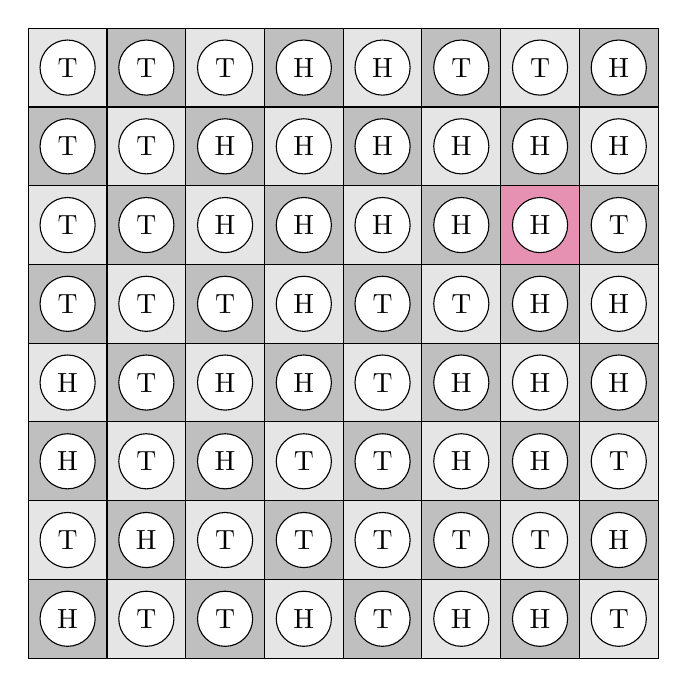
\begin{tikzpicture}[scale=1]
		\draw[fill=black, fill opacity=0.25] (0, 0) -- (0, 1) -- (1, 1) -- (1, 0) -- (0, 0);
\draw[fill=black, fill opacity=0.1] (1, 0) -- (1, 1) -- (2, 1) -- (2, 0) -- (1, 0);
\draw[fill=black, fill opacity=0.25] (2, 0) -- (2, 1) -- (3, 1) -- (3, 0) -- (2, 0);
\draw[fill=black, fill opacity=0.1] (3, 0) -- (3, 1) -- (4, 1) -- (4, 0) -- (3, 0);
\draw[fill=black, fill opacity=0.25] (4, 0) -- (4, 1) -- (5, 1) -- (5, 0) -- (4, 0);
\draw[fill=black, fill opacity=0.1] (5, 0) -- (5, 1) -- (6, 1) -- (6, 0) -- (5, 0);
\draw[fill=black, fill opacity=0.25] (6, 0) -- (6, 1) -- (7, 1) -- (7, 0) -- (6, 0);
\draw[fill=black, fill opacity=0.1] (7, 0) -- (7, 1) -- (8, 1) -- (8, 0) -- (7, 0);
\draw[fill=black, fill opacity=0.1] (0, 1) -- (0, 2) -- (1, 2) -- (1, 1) -- (0, 1);
\draw[fill=black, fill opacity=0.25] (1, 1) -- (1, 2) -- (2, 2) -- (2, 1) -- (1, 1);
\draw[fill=black, fill opacity=0.1] (2, 1) -- (2, 2) -- (3, 2) -- (3, 1) -- (2, 1);
\draw[fill=black, fill opacity=0.25] (3, 1) -- (3, 2) -- (4, 2) -- (4, 1) -- (3, 1);
\draw[fill=black, fill opacity=0.1] (4, 1) -- (4, 2) -- (5, 2) -- (5, 1) -- (4, 1);
\draw[fill=black, fill opacity=0.25] (5, 1) -- (5, 2) -- (6, 2) -- (6, 1) -- (5, 1);
\draw[fill=black, fill opacity=0.1] (6, 1) -- (6, 2) -- (7, 2) -- (7, 1) -- (6, 1);
\draw[fill=black, fill opacity=0.25] (7, 1) -- (7, 2) -- (8, 2) -- (8, 1) -- (7, 1);
\draw[fill=black, fill opacity=0.25] (0, 2) -- (0, 3) -- (1, 3) -- (1, 2) -- (0, 2);
\draw[fill=black, fill opacity=0.1] (1, 2) -- (1, 3) -- (2, 3) -- (2, 2) -- (1, 2);
\draw[fill=black, fill opacity=0.25] (2, 2) -- (2, 3) -- (3, 3) -- (3, 2) -- (2, 2);
\draw[fill=black, fill opacity=0.1] (3, 2) -- (3, 3) -- (4, 3) -- (4, 2) -- (3, 2);
\draw[fill=black, fill opacity=0.25] (4, 2) -- (4, 3) -- (5, 3) -- (5, 2) -- (4, 2);
\draw[fill=black, fill opacity=0.1] (5, 2) -- (5, 3) -- (6, 3) -- (6, 2) -- (5, 2);
\draw[fill=black, fill opacity=0.25] (6, 2) -- (6, 3) -- (7, 3) -- (7, 2) -- (6, 2);
\draw[fill=black, fill opacity=0.1] (7, 2) -- (7, 3) -- (8, 3) -- (8, 2) -- (7, 2);
\draw[fill=black, fill opacity=0.1] (0, 3) -- (0, 4) -- (1, 4) -- (1, 3) -- (0, 3);
\draw[fill=black, fill opacity=0.25] (1, 3) -- (1, 4) -- (2, 4) -- (2, 3) -- (1, 3);
\draw[fill=black, fill opacity=0.1] (2, 3) -- (2, 4) -- (3, 4) -- (3, 3) -- (2, 3);
\draw[fill=black, fill opacity=0.25] (3, 3) -- (3, 4) -- (4, 4) -- (4, 3) -- (3, 3);
\draw[fill=black, fill opacity=0.1] (4, 3) -- (4, 4) -- (5, 4) -- (5, 3) -- (4, 3);
\draw[fill=black, fill opacity=0.25] (5, 3) -- (5, 4) -- (6, 4) -- (6, 3) -- (5, 3);
\draw[fill=black, fill opacity=0.1] (6, 3) -- (6, 4) -- (7, 4) -- (7, 3) -- (6, 3);
\draw[fill=black, fill opacity=0.25] (7, 3) -- (7, 4) -- (8, 4) -- (8, 3) -- (7, 3);
\draw[fill=black, fill opacity=0.25] (0, 4) -- (0, 5) -- (1, 5) -- (1, 4) -- (0, 4);
\draw[fill=black, fill opacity=0.1] (1, 4) -- (1, 5) -- (2, 5) -- (2, 4) -- (1, 4);
\draw[fill=black, fill opacity=0.25] (2, 4) -- (2, 5) -- (3, 5) -- (3, 4) -- (2, 4);
\draw[fill=black, fill opacity=0.1] (3, 4) -- (3, 5) -- (4, 5) -- (4, 4) -- (3, 4);
\draw[fill=black, fill opacity=0.25] (4, 4) -- (4, 5) -- (5, 5) -- (5, 4) -- (4, 4);
\draw[fill=black, fill opacity=0.1] (5, 4) -- (5, 5) -- (6, 5) -- (6, 4) -- (5, 4);
\draw[fill=black, fill opacity=0.25] (6, 4) -- (6, 5) -- (7, 5) -- (7, 4) -- (6, 4);
\draw[fill=black, fill opacity=0.1] (7, 4) -- (7, 5) -- (8, 5) -- (8, 4) -- (7, 4);
\draw[fill=black, fill opacity=0.1] (0, 5) -- (0, 6) -- (1, 6) -- (1, 5) -- (0, 5);
\draw[fill=black, fill opacity=0.25] (1, 5) -- (1, 6) -- (2, 6) -- (2, 5) -- (1, 5);
\draw[fill=black, fill opacity=0.1] (2, 5) -- (2, 6) -- (3, 6) -- (3, 5) -- (2, 5);
\draw[fill=black, fill opacity=0.25] (3, 5) -- (3, 6) -- (4, 6) -- (4, 5) -- (3, 5);
\draw[fill=black, fill opacity=0.1] (4, 5) -- (4, 6) -- (5, 6) -- (5, 5) -- (4, 5);
\draw[fill=black, fill opacity=0.25] (5, 5) -- (5, 6) -- (6, 6) -- (6, 5) -- (5, 5);
\draw[fill=black, fill opacity=0.1] (6, 5) -- (6, 6) -- (7, 6) -- (7, 5) -- (6, 5);
\draw[fill=black, fill opacity=0.25] (7, 5) -- (7, 6) -- (8, 6) -- (8, 5) -- (7, 5);
\draw[fill=black, fill opacity=0.25] (0, 6) -- (0, 7) -- (1, 7) -- (1, 6) -- (0, 6);
\draw[fill=black, fill opacity=0.1] (1, 6) -- (1, 7) -- (2, 7) -- (2, 6) -- (1, 6);
\draw[fill=black, fill opacity=0.25] (2, 6) -- (2, 7) -- (3, 7) -- (3, 6) -- (2, 6);
\draw[fill=black, fill opacity=0.1] (3, 6) -- (3, 7) -- (4, 7) -- (4, 6) -- (3, 6);
\draw[fill=black, fill opacity=0.25] (4, 6) -- (4, 7) -- (5, 7) -- (5, 6) -- (4, 6);
\draw[fill=black, fill opacity=0.1] (5, 6) -- (5, 7) -- (6, 7) -- (6, 6) -- (5, 6);
\draw[fill=black, fill opacity=0.25] (6, 6) -- (6, 7) -- (7, 7) -- (7, 6) -- (6, 6);
\draw[fill=black, fill opacity=0.1] (7, 6) -- (7, 7) -- (8, 7) -- (8, 6) -- (7, 6);
\draw[fill=black, fill opacity=0.1] (0, 7) -- (0, 8) -- (1, 8) -- (1, 7) -- (0, 7);
\draw[fill=black, fill opacity=0.25] (1, 7) -- (1, 8) -- (2, 8) -- (2, 7) -- (1, 7);
\draw[fill=black, fill opacity=0.1] (2, 7) -- (2, 8) -- (3, 8) -- (3, 7) -- (2, 7);
\draw[fill=black, fill opacity=0.25] (3, 7) -- (3, 8) -- (4, 8) -- (4, 7) -- (3, 7);
\draw[fill=black, fill opacity=0.1] (4, 7) -- (4, 8) -- (5, 8) -- (5, 7) -- (4, 7);
\draw[fill=black, fill opacity=0.25] (5, 7) -- (5, 8) -- (6, 8) -- (6, 7) -- (5, 7);
\draw[fill=black, fill opacity=0.1] (6, 7) -- (6, 8) -- (7, 8) -- (7, 7) -- (6, 7);
\draw[fill=black, fill opacity=0.25] (7, 7) -- (7, 8) -- (8, 8) -- (8, 7) -- (7, 7);

\draw[fill=WildStrawberry, fill opacity=0.4] (6, 5) -- (6, 6) -- (7, 6) -- (7, 5) -- (6, 5);

\draw[fill=white, fill opacity=1](0.5, 0.5) circle (0.35);
\node at (0.5, 0.5) {H};
\draw[fill=white, fill opacity=1](1.5, 0.5) circle (0.35);
\node at (1.5, 0.5) {T};
\draw[fill=white, fill opacity=1](2.5, 0.5) circle (0.35);
\node at (2.5, 0.5) {T};
\draw[fill=white, fill opacity=1](3.5, 0.5) circle (0.35);
\node at (3.5, 0.5) {H};
\draw[fill=white, fill opacity=1](4.5, 0.5) circle (0.35);
\node at (4.5, 0.5) {T};
\draw[fill=white, fill opacity=1](5.5, 0.5) circle (0.35);
\node at (5.5, 0.5) {H};
\draw[fill=white, fill opacity=1](6.5, 0.5) circle (0.35);
\node at (6.5, 0.5) {H};
\draw[fill=white, fill opacity=1](7.5, 0.5) circle (0.35);
\node at (7.5, 0.5) {T};
\draw[fill=white, fill opacity=1](0.5, 1.5) circle (0.35);
\node at (0.5, 1.5) {T};
\draw[fill=white, fill opacity=1](1.5, 1.5) circle (0.35);
\node at (1.5, 1.5) {H};
\draw[fill=white, fill opacity=1](2.5, 1.5) circle (0.35);
\node at (2.5, 1.5) {T};
\draw[fill=white, fill opacity=1](3.5, 1.5) circle (0.35);
\node at (3.5, 1.5) {T};
\draw[fill=white, fill opacity=1](4.5, 1.5) circle (0.35);
\node at (4.5, 1.5) {T};
\draw[fill=white, fill opacity=1](5.5, 1.5) circle (0.35);
\node at (5.5, 1.5) {T};
\draw[fill=white, fill opacity=1](6.5, 1.5) circle (0.35);
\node at (6.5, 1.5) {T};
\draw[fill=white, fill opacity=1](7.5, 1.5) circle (0.35);
\node at (7.5, 1.5) {H};
\draw[fill=white, fill opacity=1](0.5, 2.5) circle (0.35);
\node at (0.5, 2.5) {H};
\draw[fill=white, fill opacity=1](1.5, 2.5) circle (0.35);
\node at (1.5, 2.5) {T};
\draw[fill=white, fill opacity=1](2.5, 2.5) circle (0.35);
\node at (2.5, 2.5) {H};
\draw[fill=white, fill opacity=1](3.5, 2.5) circle (0.35);
\node at (3.5, 2.5) {T};
\draw[fill=white, fill opacity=1](4.5, 2.5) circle (0.35);
\node at (4.5, 2.5) {T};
\draw[fill=white, fill opacity=1](5.5, 2.5) circle (0.35);
\node at (5.5, 2.5) {H};
\draw[fill=white, fill opacity=1](6.5, 2.5) circle (0.35);
\node at (6.5, 2.5) {H};
\draw[fill=white, fill opacity=1](7.5, 2.5) circle (0.35);
\node at (7.5, 2.5) {T};
\draw[fill=white, fill opacity=1](0.5, 3.5) circle (0.35);
\node at (0.5, 3.5) {H};
\draw[fill=white, fill opacity=1](1.5, 3.5) circle (0.35);
\node at (1.5, 3.5) {T};
\draw[fill=white, fill opacity=1](2.5, 3.5) circle (0.35);
\node at (2.5, 3.5) {H};
\draw[fill=white, fill opacity=1](3.5, 3.5) circle (0.35);
\node at (3.5, 3.5) {H};
\draw[fill=white, fill opacity=1](4.5, 3.5) circle (0.35);
\node at (4.5, 3.5) {T};
\draw[fill=white, fill opacity=1](5.5, 3.5) circle (0.35);
\node at (5.5, 3.5) {H};
\draw[fill=white, fill opacity=1](6.5, 3.5) circle (0.35);
\node at (6.5, 3.5) {H};
\draw[fill=white, fill opacity=1](7.5, 3.5) circle (0.35);
\node at (7.5, 3.5) {H};
\draw[fill=white, fill opacity=1](0.5, 4.5) circle (0.35);
\node at (0.5, 4.5) {T};
\draw[fill=white, fill opacity=1](1.5, 4.5) circle (0.35);
\node at (1.5, 4.5) {T};
\draw[fill=white, fill opacity=1](2.5, 4.5) circle (0.35);
\node at (2.5, 4.5) {T};
\draw[fill=white, fill opacity=1](3.5, 4.5) circle (0.35);
\node at (3.5, 4.5) {H};
\draw[fill=white, fill opacity=1](4.5, 4.5) circle (0.35);
\node at (4.5, 4.5) {T};
\draw[fill=white, fill opacity=1](5.5, 4.5) circle (0.35);
\node at (5.5, 4.5) {T};
\draw[fill=white, fill opacity=1](6.5, 4.5) circle (0.35);
\node at (6.5, 4.5) {H};
\draw[fill=white, fill opacity=1](7.5, 4.5) circle (0.35);
\node at (7.5, 4.5) {H};
\draw[fill=white, fill opacity=1](0.5, 5.5) circle (0.35);
\node at (0.5, 5.5) {T};
\draw[fill=white, fill opacity=1](1.5, 5.5) circle (0.35);
\node at (1.5, 5.5) {T};
\draw[fill=white, fill opacity=1](2.5, 5.5) circle (0.35);
\node at (2.5, 5.5) {H};
\draw[fill=white, fill opacity=1](3.5, 5.5) circle (0.35);
\node at (3.5, 5.5) {H};
\draw[fill=white, fill opacity=1](4.5, 5.5) circle (0.35);
\node at (4.5, 5.5) {H};
\draw[fill=white, fill opacity=1](5.5, 5.5) circle (0.35);
\node at (5.5, 5.5) {H};
\draw[fill=white, fill opacity=1](6.5, 5.5) circle (0.35);
\node at (6.5, 5.5) {H};
\draw[fill=white, fill opacity=1](7.5, 5.5) circle (0.35);
\node at (7.5, 5.5) {T};
\draw[fill=white, fill opacity=1](0.5, 6.5) circle (0.35);
\node at (0.5, 6.5) {T};
\draw[fill=white, fill opacity=1](1.5, 6.5) circle (0.35);
\node at (1.5, 6.5) {T};
\draw[fill=white, fill opacity=1](2.5, 6.5) circle (0.35);
\node at (2.5, 6.5) {H};
\draw[fill=white, fill opacity=1](3.5, 6.5) circle (0.35);
\node at (3.5, 6.5) {H};
\draw[fill=white, fill opacity=1](4.5, 6.5) circle (0.35);
\node at (4.5, 6.5) {H};
\draw[fill=white, fill opacity=1](5.5, 6.5) circle (0.35);
\node at (5.5, 6.5) {H};
\draw[fill=white, fill opacity=1](6.5, 6.5) circle (0.35);
\node at (6.5, 6.5) {H};
\draw[fill=white, fill opacity=1](7.5, 6.5) circle (0.35);
\node at (7.5, 6.5) {H};
\draw[fill=white, fill opacity=1](0.5, 7.5) circle (0.35);
\node at (0.5, 7.5) {T};
\draw[fill=white, fill opacity=1](1.5, 7.5) circle (0.35);
\node at (1.5, 7.5) {T};
\draw[fill=white, fill opacity=1](2.5, 7.5) circle (0.35);
\node at (2.5, 7.5) {T};
\draw[fill=white, fill opacity=1](3.5, 7.5) circle (0.35);
\node at (3.5, 7.5) {H};
\draw[fill=white, fill opacity=1](4.5, 7.5) circle (0.35);
\node at (4.5, 7.5) {H};
\draw[fill=white, fill opacity=1](5.5, 7.5) circle (0.35);
\node at (5.5, 7.5) {T};
\draw[fill=white, fill opacity=1](6.5, 7.5) circle (0.35);
\node at (6.5, 7.5) {T};
\draw[fill=white, fill opacity=1](7.5, 7.5) circle (0.35);
\node at (7.5, 7.5) {H};
	\end{tikzpicture}
	\caption{An example of random coins on a chessboard. The red highlighted square indicates the position of the key.}
	\label{fig:TheChessboardEncodingProblem_Example}
\end{figure}

\begin{table}[H]
	\centering
	\caption{An example of how to determine which regions to flip the parity of}
	\label{tab:TheChessboardEncodingProblem_ExampleParity}
	\begin{tabular}{cccccc}
		\myhline
		Region & Head Count & Head Parity & Encoded Parity & Parity Change & Flip Red Region  \\
		\myhline
		\tableinput{1 - Logic/TheChessboardEncodingProblem/ChessboardExampleTable.tex}
		\myhline
	\end{tabular}
\end{table}

Reading from the last column, we need to flip the coin with encoding 001011 which is the the second column and third row. Once this is done, the parities of the different regions would be read off as 111011, precisely giving the position of the square with the hidden key. Note that the position of the coin to flip is given by the XOR of the state encoded by the position of the hidden key and the state encoded by the board.

\textbf{Extensions and Comments:}

We notice that as there are $2^6$ different states to encode and $2^{64}$ boards, there must be $2^6$ sets of $2^{58}$ elements that are equivalent in some sense. We can make this intuition more rigorous. Consider the set of 64-tuples of binary numbers, $G = \{ 0, 1 \}^{64}$. For $x, y \in G$ we can define the binary option, $x \circ y := (x + y) \mod 2$, and note that this is equivalent to elementwise XOR. This can easily be seen to form an abelian group. Elements of this group represent states of the board. We can also make a group where each element corresponds to a square on the board.

Define $f(x)$ to be the function that takes $x$ to the index of the cell that it encodes. With an abuse of notation using $\sum$ to mean repeated application of $\circ$, we can give this function explicitly as $f(x) = \sum_{i \in I_k} x_i$ where $I_k$ is the indexing set corresponding to the $k^\text{th}$ digit in the encoding. If we define $K := \ker{f}$ then it follows from the first isomorphism theorem that $K$ is a normal subgroup of $G$ and the quotient group $H = G / K$ is well-defined. $K$ represents all the board states that encode $0$ and we are dividing out this information. This means that we expect each element of $H$ to represent all the board states that encodes the same square.

We could arrive at the same group through a congruence. Define an equivalence relation between board states where two states are equivalent if they encode the same cell, that is, $x \sim y \iff f(x) = f(y)$. It is easy to show this is an equivalence as the equivalency axioms are inherited from the equality relation. Equation~\eqref{eqn:TheChessboardEncodingProblem_SelfInverse} demonstrates that mapped elements are self-inverse from which if follows in equation~\eqref{eqn:TheChessboardEncodingProblem_CongruenceRespectsInverses} that the congruence relation respects inverses. Equation \eqref{eqn:TheChessboardEncodingProblem_LinearityOfF} shows that $f$ is linear and thus the congruence respects the binary operation as well, as shown in \eqref{eqn:TheChessboardEncodingProblem_CongruenceRespectsProducts}. This is essentially equivalent to saying that flipping the parity of a coin within a region flips the parity of the whole region.

\begin{subequations}
	\begin{align}
	\begin{split}
		f(x) \circ f(x) = 0 &\implies f(x) = f(x)^{-1}
		\label{eqn:TheChessboardEncodingProblem_SelfInverse}
	\end{split}\\
	\begin{split}
		f(x) = f(y) &\implies f(x)^{-1} = f(y)^{-1}
		\label{eqn:TheChessboardEncodingProblem_CongruenceRespectsInverses}
	\end{split}\\
	\begin{split}
		f(x)_k \circ f(y)_k = \sum_{i \in I_k} x_i \circ \sum_{i \in I_k} y_i &= \sum_{i \in I_k} x_i \circ y_i = \sum_{i \in I_k} (x \circ y)_i = f(x \circ y)_k
		\label{eqn:TheChessboardEncodingProblem_LinearityOfF}
	\end{split}
	\end{align}
	
	\begin{equation}
		\begin{aligned}
			x^1 \sim y^1,\, x^2 \sim y^2 &\implies f(x^1) = f(y^1),\, f(x^2) = f(y^2)  \\
			&\implies f(x^1 \circ x^2)_k = f(x^1) \circ f(x^2) = f(y^1) \circ f(y^2) = f(y^1 \circ y^2)  \\
			&\implies x^1 \circ x^2 \sim y^1 \circ y^2
		\end{aligned}
		\label{eqn:TheChessboardEncodingProblem_CongruenceRespectsProducts}
	\end{equation}
\end{subequations}